\section{Introducción}

Luego de haber estudiado los conceptos de aritmética de \emph{punto fijo}, se propuso como trabajo generar filtros de \emph{coseno realzado} (RC) en distintos formatos de punto fijo, para comparar cómo la cuantización afecta su desempeño a la hora de limitar el ancho de banda de un canal.

\section{Desarrollo}

\subsection{Filtros en Punto Flotante}

Se diseñaron en Python tres filtros RC con Rolloff 0, $0.5$ y 1. Estos están en punto flotante para determinar sus diferencias antes de cuantizarlos, y las características que comparten son:

\begin{itemize}
    \item $BR$ (Baudrate) $= 1\,$GBd
    \item Duración: 16 períodos de baudio.
    \item $OS$ (Oversampling) $= 8$
\end{itemize}

En la figura \ref{fig:imp_float} se muestra la respuesta al impulso de los filtros. Así como se observó en el trabajo práctico N°1, se observa que los lóbulos de un filtro con rolloff menor decaen más lento en amplitud, por lo que se requiere un mayor número de coeficientes. También cruzan por cero en múltiplos del período de símbolo $T$, lo que les da la capacidad de eliminación de I.S.I.

En la figura \ref{fig:freq_float} se puede observar la respuesta en frecuencia utilizando la función \texttt{fft} de numpy y normalizando los filtros en amplitud para que tengan ganancia de $0\,$dB en la banda de paso. Se observa la transición abrupta en $\beta=0$, pero con una atenuación pobre fuera de banda, ya que los lóbulos laterales en el tiempo no se terminan de extinguir; mientras que con rolloff más alto, la transición es más suave (ocupando más ancho de banda) pero atenúa mejor fuera de banda. Se debe tener en cuenta que, en este caso, los lóbulos en la banda de atenuación se ven más ``prolijos'' que en el caso de un filtro en punto fijo, como se verá más adelante.

\begin{figure}[H]
    \centering
    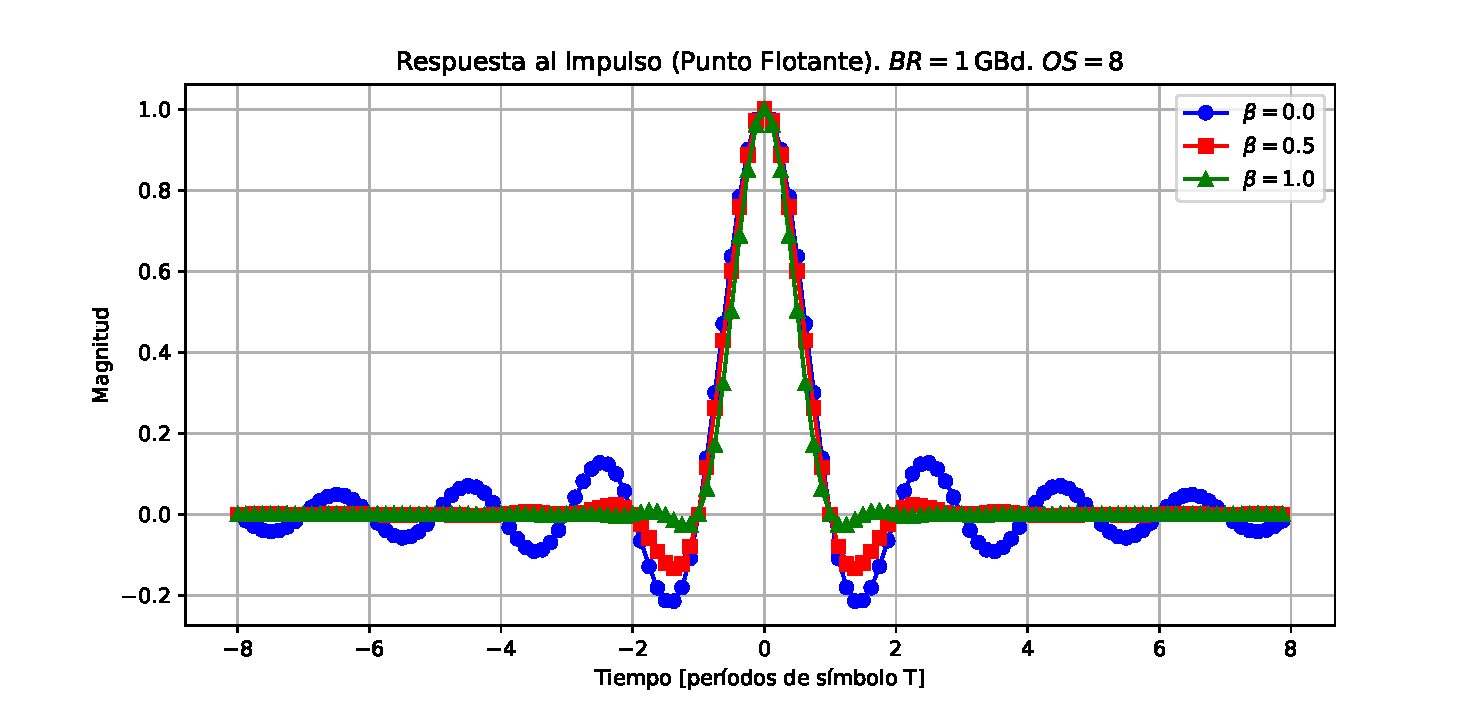
\includegraphics[width=\linewidth]{img/imp_float.pdf}
    \caption{Respuesta al impulso de los filtros en punto flotante.}
    \label{fig:imp_float}
\end{figure}

\begin{figure}[H]
    \centering
    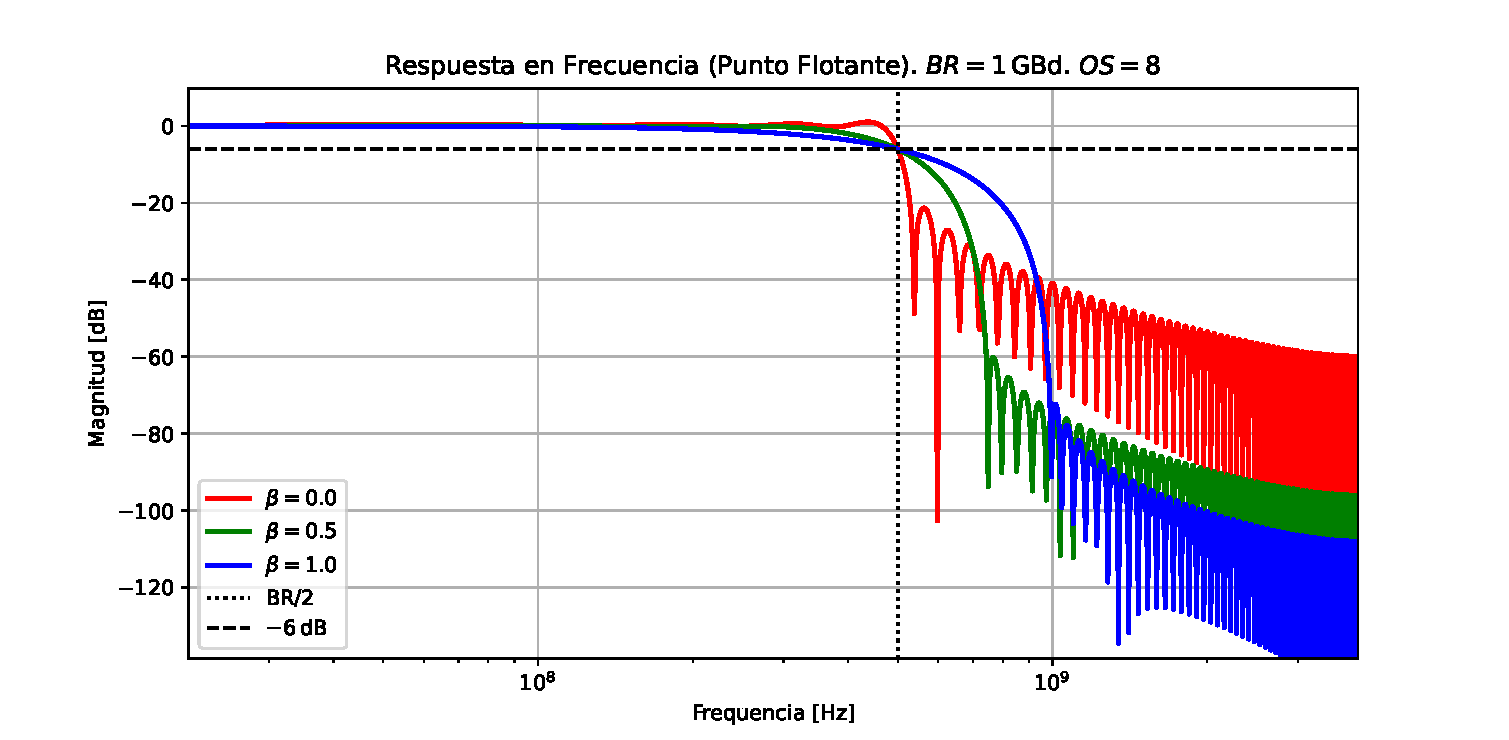
\includegraphics[width=\linewidth]{img/freq_float.pdf}
    \caption{Respuesta en frecuencia de los filtros normalizados en punto flotante.}
    \label{fig:freq_float}
\end{figure}

Durante la transmisión, el DSP realiza la convolución del RC con los símbolos a enviar. En Python se graficó la convolución de dos símbolos con estos tres filtros en la figura \ref{fig:conv_float}; como estos símbolos son un impulso, de la convolución se obtuvo la suma de dos RC, donde la suma se encuentra en color azul. La diferencia que se observa entre los distintos $\beta$, es que con un $\beta$ muy bajo se produce una señal de larga duración y muy oscilante, mientras que con un $\beta$ bajo, la señal es de menor duración y menos oscilante.

Finalmente, se generaron varios símbolos en un esquema de modulación QPSK y se los filtró con los tres RC de punto flotante anteriores. Luego se graficó la \emph{constelación} resultante con la fase óptima en la figura \ref{fig:const_float}. Una constelación es un diagrama que representa los símbolos recibidos muestreados en el instante óptimo de decisión. En ese instante, todos los filtros RC —sin importar el valor de $\beta$— cumplen el criterio para I.S.I. cero y el valor muestreado corresponde únicamente al símbolo transmitido.

\begin{figure}[H]
    \centering
    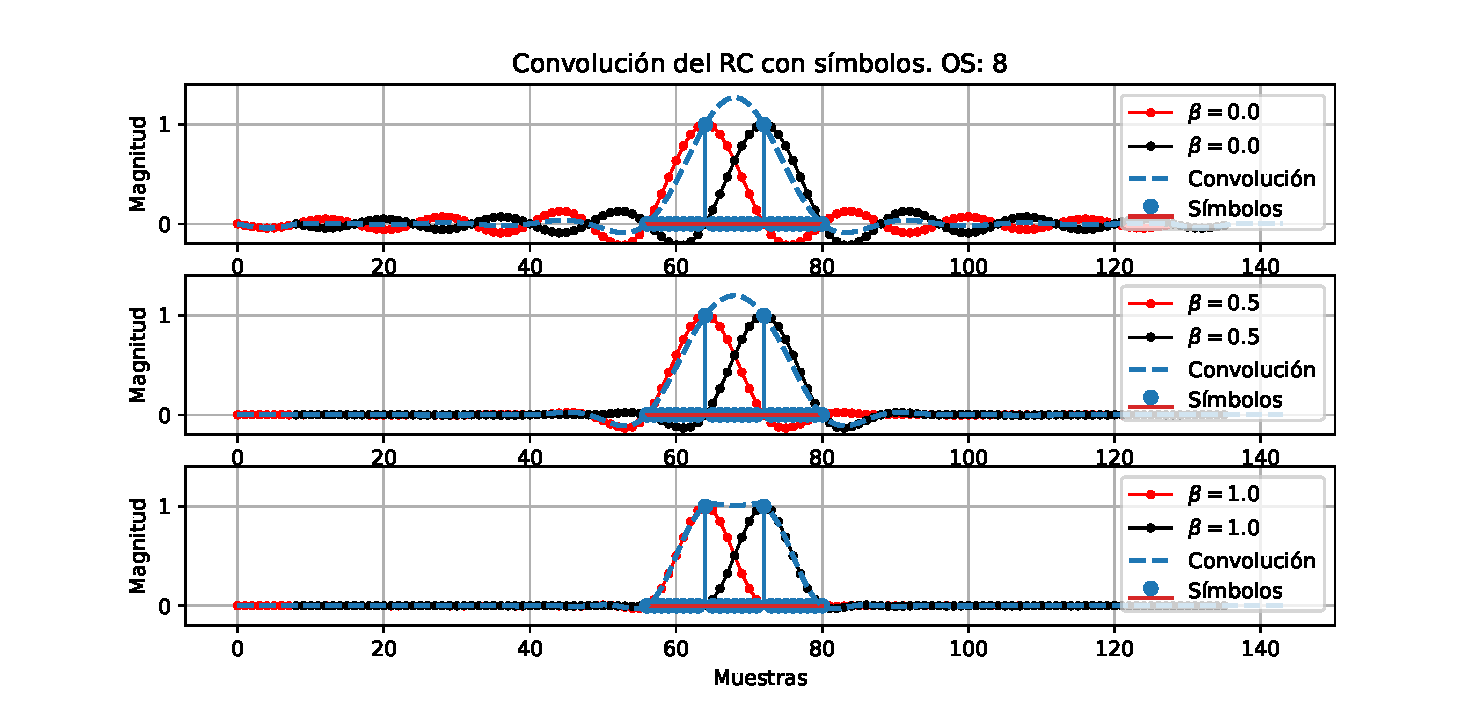
\includegraphics[width=\linewidth]{img/conv_float.pdf}
    \caption{Convolución de los tres filtros con dos símbolos.}
    \label{fig:conv_float}
\end{figure}

\begin{figure}[H]
    \centering
    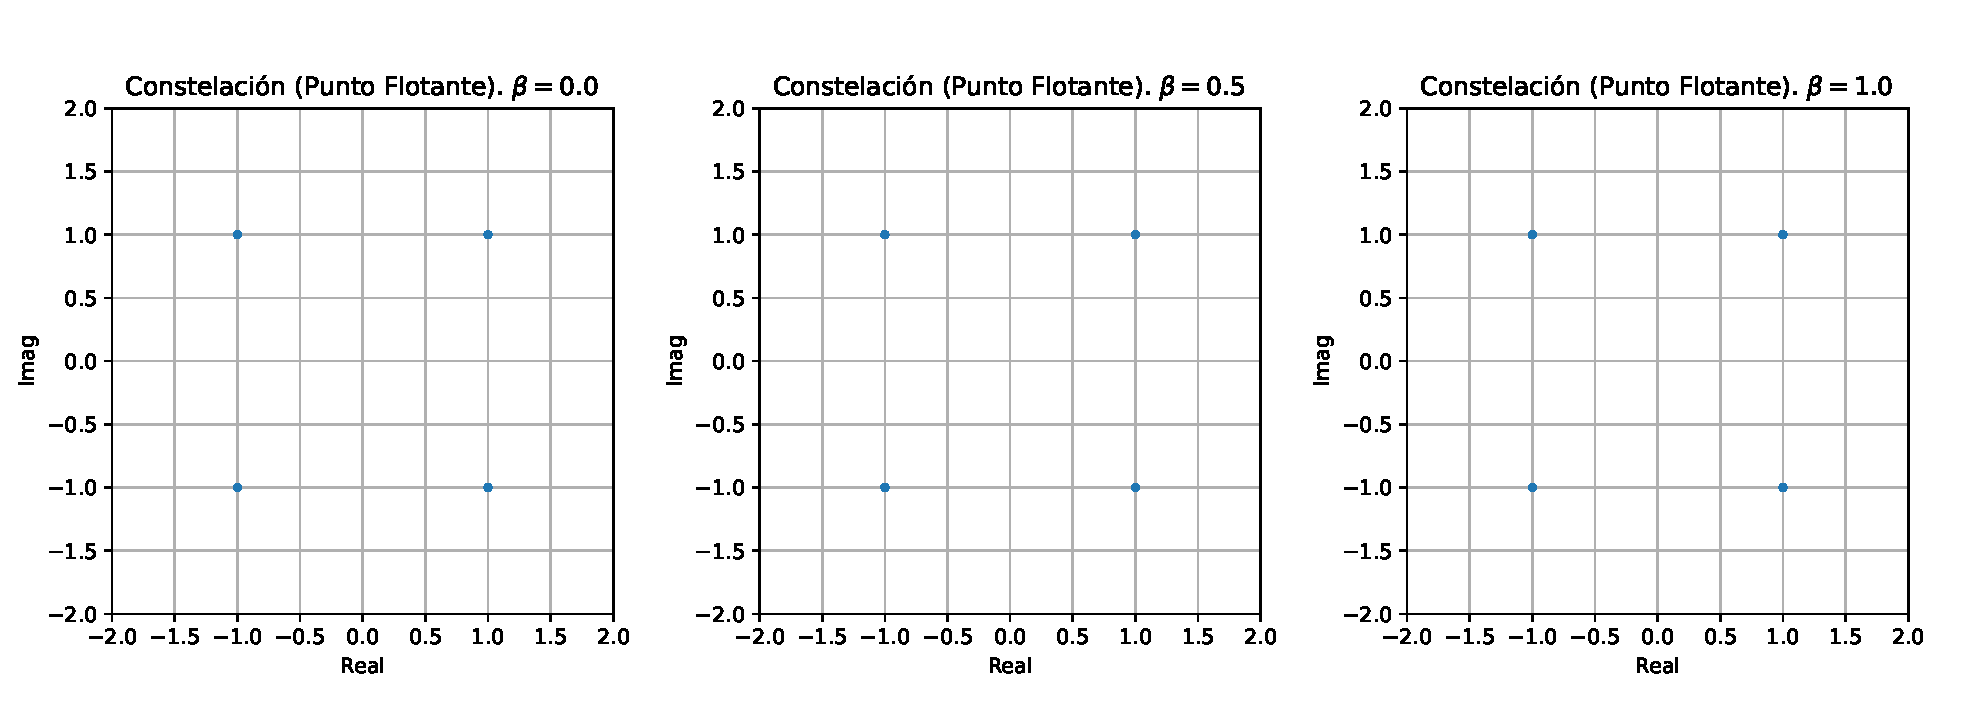
\includegraphics[width=\linewidth]{img/const_float.pdf}
    \caption{Diagrama de constelación para los filtros en punto flotante. Modulación QPSK.}
    \label{fig:const_float}
\end{figure}

Por lo tanto, el factor de rolloff no influye en la posición de los puntos de la constelación cuando el filtro está en formato de punto flotante.

\subsection{Filtros en Punto Fijo}

Para esta sección, los filtros de punto flotante anteriores fueron cuantizados en los siguientes formatos de punto fijo:

\begin{itemize}
    \item S(8,7): valores signados de 8 bits en total y 7 bits fraccionales.
    \item S(6,4): valores signados de 6 bits en total y 4 bits fraccionales.
    \item S(3,2): valores signados de 3 bits en total y 2 bits fraccionales.
\end{itemize}

Para poder acortar la representación en 32 bits del punto flotante a la cantidad de bits correspondientes del punto fijo, se realizó la conversión aplicando \emph{saturación} para que no haya overflow en valores altos y aplicando también los métodos de \emph{truncado} y \emph{redondeo}. Estos dos últimos consisten en lo siguiente:

\begin{itemize}
    \item \textbf{Truncado}: los bits fraccionales a eliminar directamente se descartan y se conserva la cantidad de bits deseada.
    \item \textbf{Redondeo no simétrico}: al valor sin truncar se le suma siempre un 1 en la posición del bit más significativo a eliminar, luego se lo trunca.
    \item \textbf{Redondeo simétrico}: ídem al redondeo no simétrico, solo que se suma 1 si el número es positivo y se resta 1 si es negativo (\emph{redondeo hacia infinito}), o viceversa (\emph{redondeo hacia cero}).
\end{itemize}

Se resumieron algunas características de los formatos en el cuadro \ref{tab:formatos}.

\begin{table}[H]
    \centering

    \begin{tabular}{lccc}
        \textbf{Formato} & \textbf{Precisión} & \textbf{Resolución} & \textbf{Rango} \\
        \hline\hline
        \textbf{S(8,7)} & 8 bits (256 valores) & $0.0078125$ & $[-1:0.9921875]$ \\
        \textbf{S(6,4)} & 6 bits (64 valores)  & $0.0625$    & $[-2:1.9375]$    \\
        \textbf{S(3,2)} & 3 bits (8 valores)   & $0.25$      & $[-1:0.75]$      \\
        \hline
    \end{tabular}

    \caption{Comparación entre tres formatos de punto fijo.}
    \label{tab:formatos}
\end{table}

Cabe aclarar que, a diferencia de los filtros en punto flotante, en este caso no se normalizaron para ver su respuesta en frecuencia, ya que esto implicaría tener una menor resolución final.

En la figura \ref{fig:imp_fix_beta05} se muestra una comparación entre estos tres formatos. Nótese que los filtros en S(8,7) y S(3,2) no llegan a 1 en el lóbulo principal, ya que se encuentran limitados por su rango de valores representables, mostrados en el cuadro \ref{tab:formatos}. Además, se observa que los filtros de menor precisión S(6,4) y S(3,2) difieren más de los valores ideales de punto flotante, ya que al tener menor precisión tienen también menor resolución.

La respuesta en frecuencia de estos filtros en la figura \ref{fig:freq_fix_beta05} evidencia que una resolución muy baja implica una respuesta más pobre en frecuencia. El filtro en S(3,2) es diferente incluso en la banda de paso, por lo que no sería útil en la práctica. Por otro lado, el filtro en S(6,4) sigue un poco mejor a la respuesta ideal, pero en la banda de paso tiene una ganancia distinta. El filtro S(8,7) es el que mejor sigue al ideal, aunque fuera de banda hay poca atenuación.

\begin{figure}[H]
    \centering
    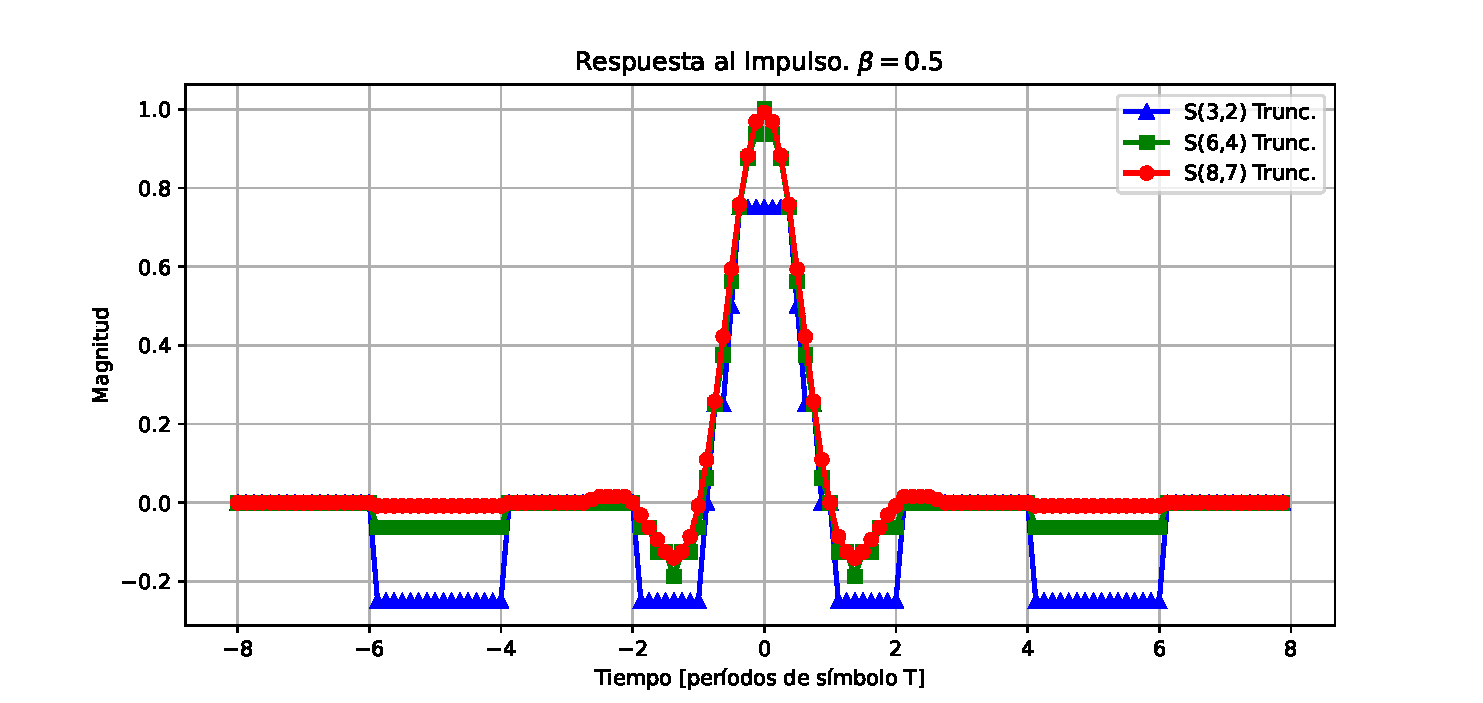
\includegraphics[width=\linewidth]{img/imp_fix_beta05.pdf}
    \caption{Respuesta al impulso de un RC en punto fijo, con truncado.}
    \label{fig:imp_fix_beta05}
\end{figure}

\begin{figure}[H]
    \centering
    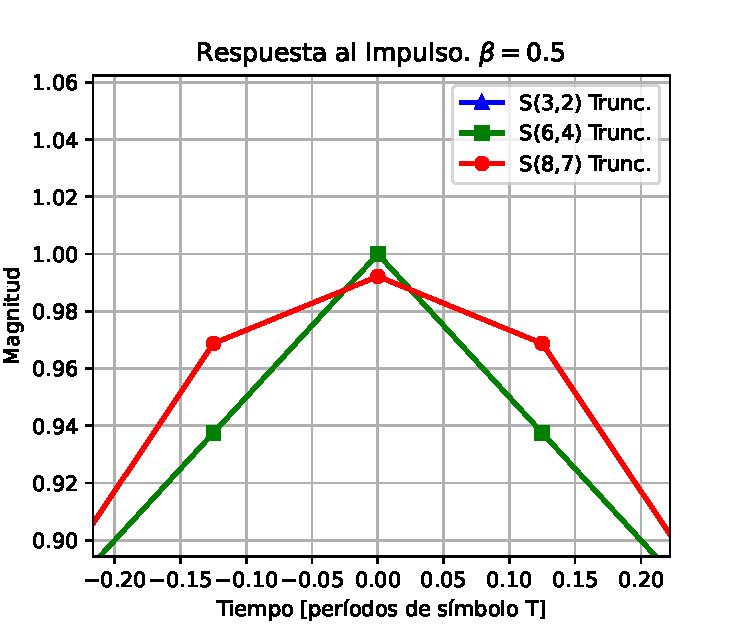
\includegraphics[width=0.4\linewidth]{img/imp_fix_beta05_2.pdf}
    \caption{Acercamiento al lóbulo principal de la respuesta. El coeficiente en S(8,7) no llega a 1.}
    \label{fig:imp_fix_beta05_2}
\end{figure}

\begin{figure}[H]
    \centering
    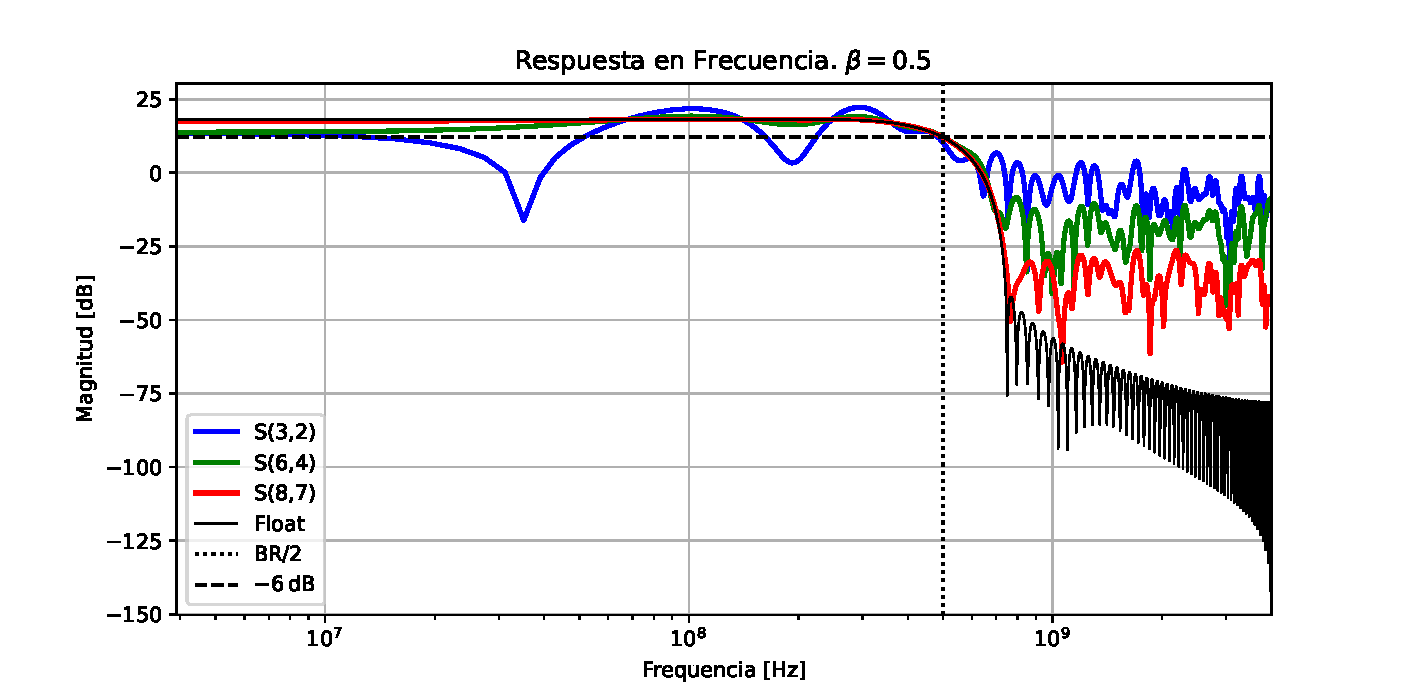
\includegraphics[width=\linewidth]{img/freq_fix_beta05.pdf}
    \caption{Respuesta en frecuencia de un RC en punto fijo, con truncado.}
    \label{fig:freq_fix_beta05}
\end{figure}

En la figura \ref{fig:imp_fix_s64} se compararon los distintos factores de rolloff en un filtro cuantizado, observándose que para un rolloff de 1 los lóbulos laterales no se terminan de extinguir. Esto provoca que el filtro no pueda atenuar altas frecuencias, como se observa en la figura \ref{fig:freq_fix_s64}, donde la atenuación para este caso es la misma. Se concluye entonces que, para baja resolución, la atenuación en altas frecuencias depende del formato de punto fijo y no necesariamente del rolloff.

\begin{figure}[H]
    \centering
    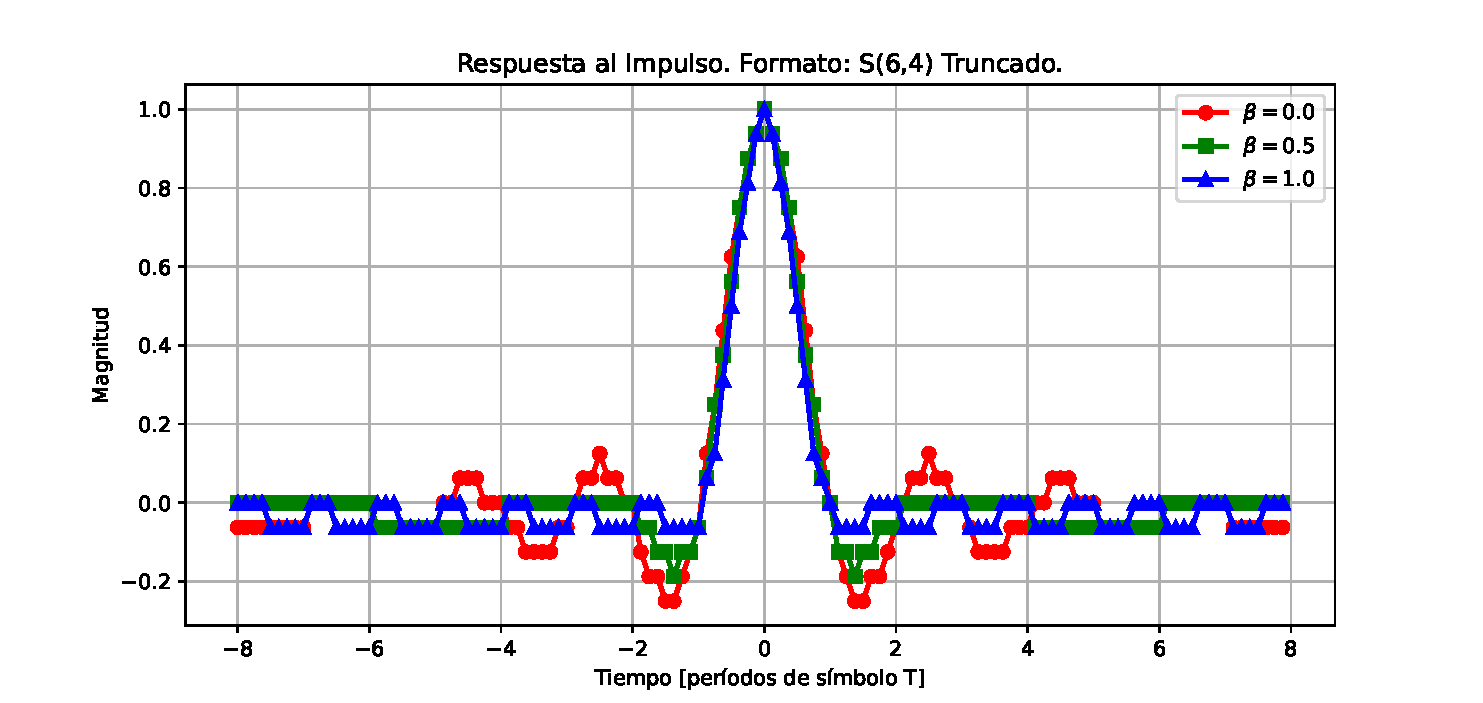
\includegraphics[width=\linewidth]{img/imp_fix_s64.pdf}
    \caption{Respuesta al impulso de un RC en punto fijo según el rolloff.}
    \label{fig:imp_fix_s64}
\end{figure}

\begin{figure}[H]
    \centering
    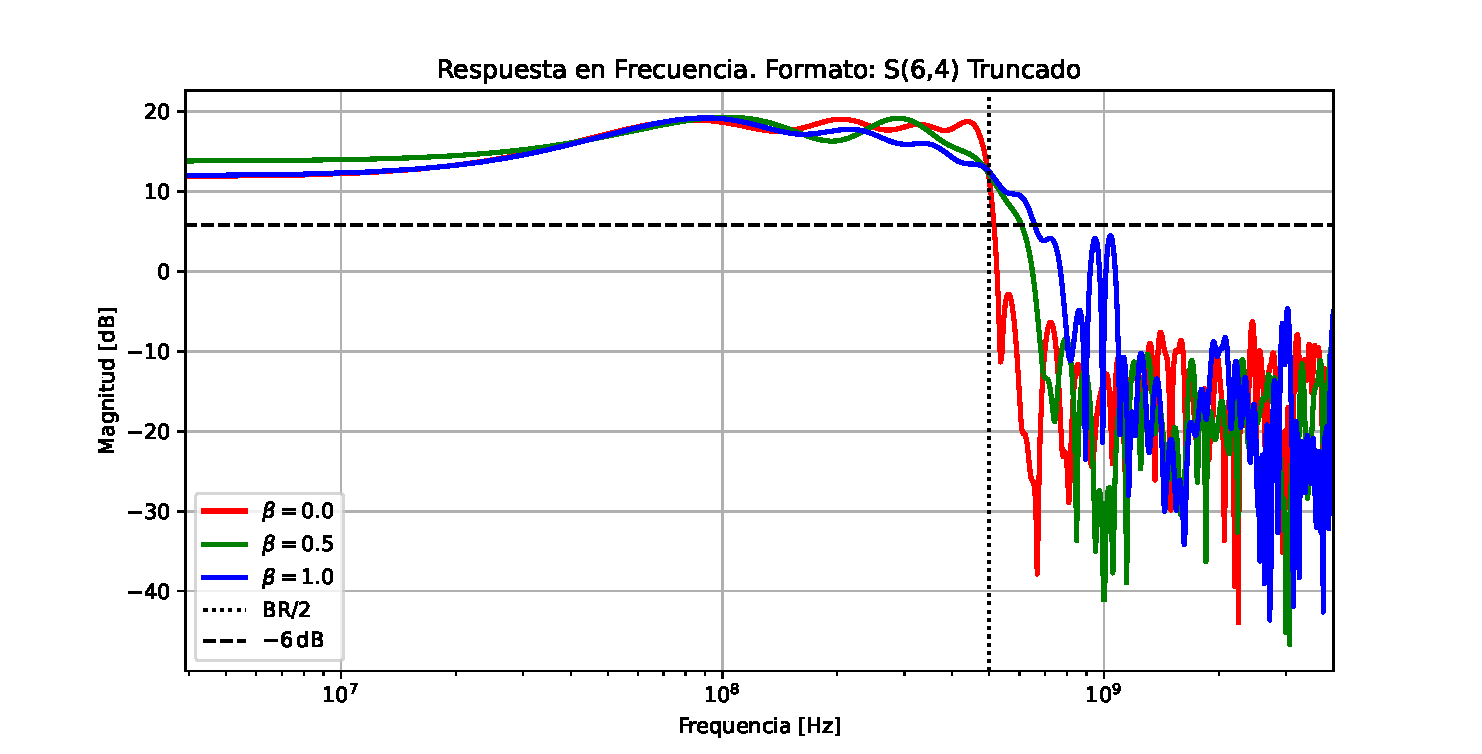
\includegraphics[width=\linewidth]{img/freq_fix_s64.pdf}
    \caption{Respuesta en frecuencia de un RC en punto fijo según el rolloff.}
    \label{fig:freq_fix_s64}
\end{figure}

Nuevamente prestando atención a un rolloff de 1, la diferencia entre un filtro en punto fijo con truncado y uno con redondeo se muestra en la figura \ref{fig:imp_fix_trunc_red_beta1}. La clase de python utilizada, \texttt{\_fixedInt.py}, utiliza un redondeo simétrico hacia cero.

Se puede observar detenidamente que el filtro con truncado no es simétrico, mientras que el filtro con redondeo sí lo es. Esto, sumado a que los coeficientes sí se extinguen en este caso, se espera la respuesta en frecuencia de la figura \ref{fig:freq_fix_trunc_red_beta1}; la respuesta con redondeo tiene mejor atenuación, ya que los lóbulos laterales son directamente cero y no oscilan, mientras que la banda de paso es contante. Se puede deducir que si a los coeficientes se les aplica un redondeo no simétrico (siempre se suma 1 al bit más significativo a truncar)

\begin{figure}[H]
    \centering
    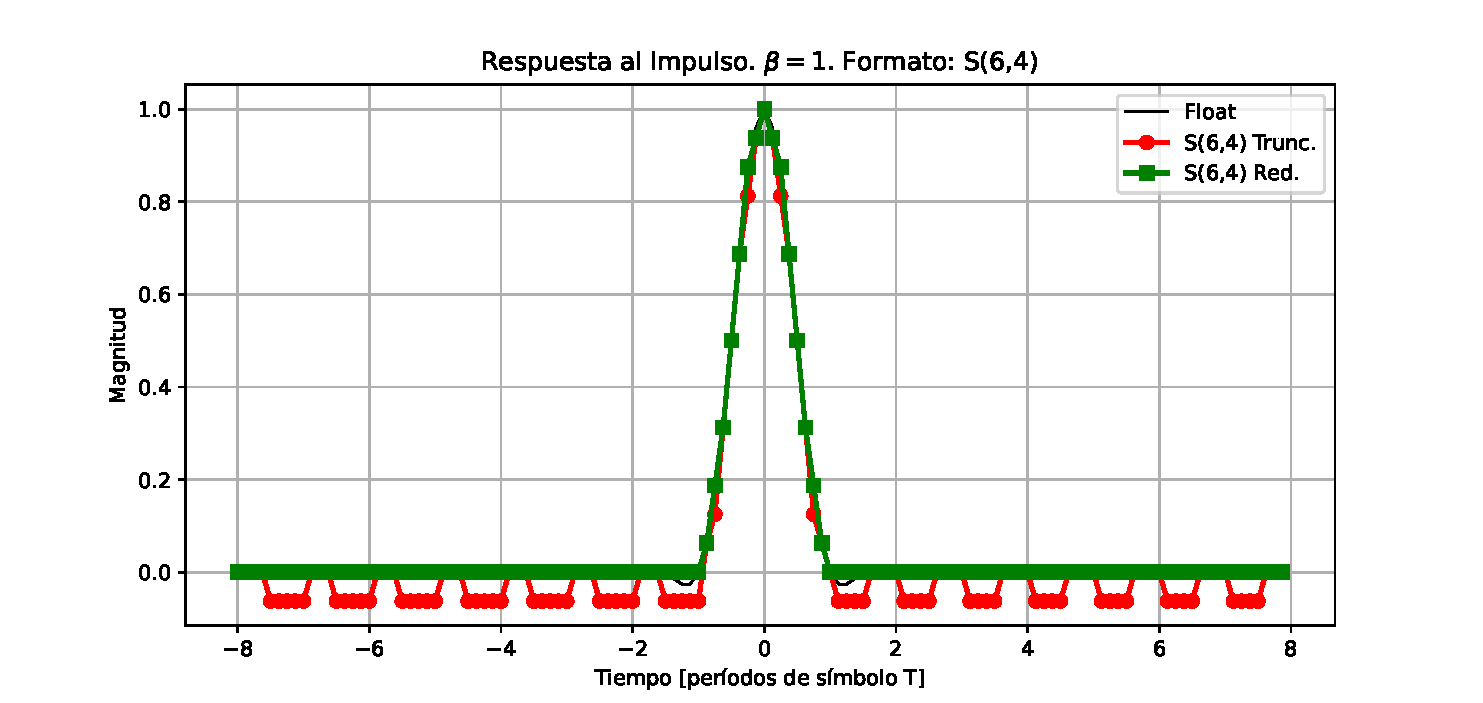
\includegraphics[width=\linewidth]{img/imp_fix_trunc_red_beta1.pdf}
    \caption{Respuesta al impulso de un filtro con truncado y uno con redondeo.}
    \label{fig:imp_fix_trunc_red_beta1}
\end{figure}

\begin{figure}[H]
    \centering
    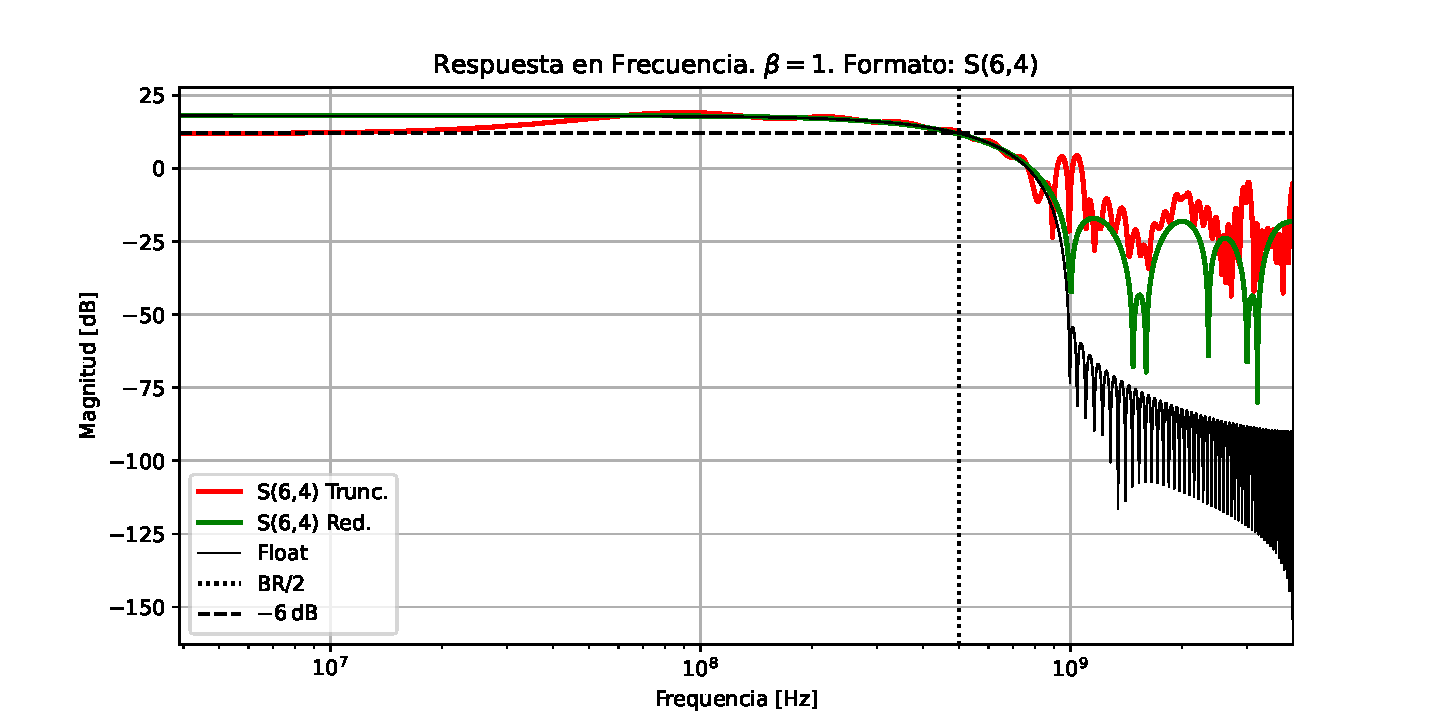
\includegraphics[width=\linewidth]{img/freq_fix_trunc_red_beta1.pdf}
    \caption{Respuesta en frecuencia de un filtro con truncado y uno con redondeo.}
    \label{fig:freq_fix_trunc_red_beta1}
\end{figure}

En la figura \ref{fig:imp_fix_beta05_round} se puede ver una comparación entre los tres formatos con redondeo donde los coeficientes son simétricos, a diferencia de la figura \ref{fig:imp_fix_beta05}. La respuesta en frecuencia en la figura \ref{fig:freq_fix_beta05_round} también muestra una mejora en la banda de paso, comparado con la figura \ref{fig:freq_fix_beta05}. Observando todas estas diferencias, se deduce que un filtro con redondeo tiene un mejor comportamiento respecto a uno con truncado, por lo que en la práctica es más frecuente el uso del redondeo en la conversión.

\begin{figure}[H]
    \centering
    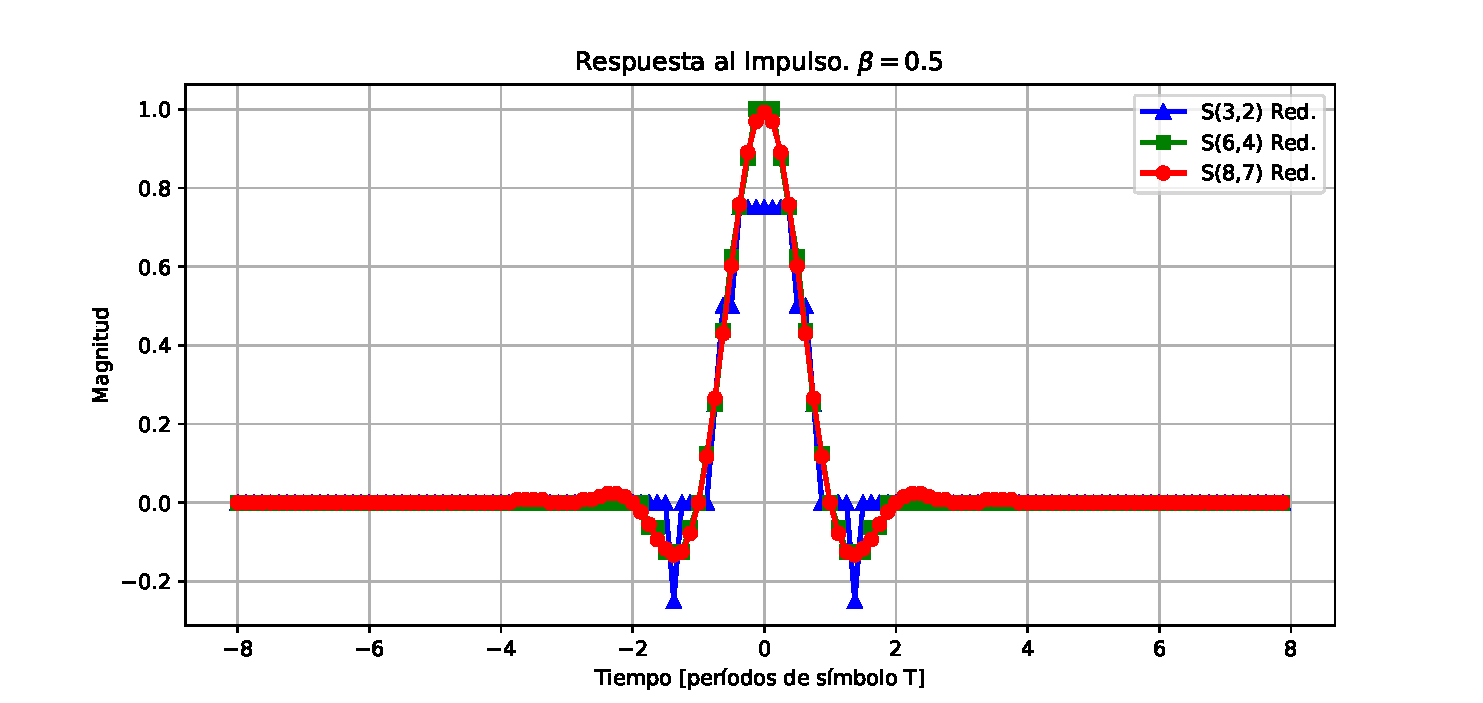
\includegraphics[width=\linewidth]{img/imp_fix_beta05_round.pdf}
    \caption{Respuesta al impulso del RC en punto fijo, con redondeo.}
    \label{fig:imp_fix_beta05_round}
\end{figure}

\begin{figure}[H]
    \centering
    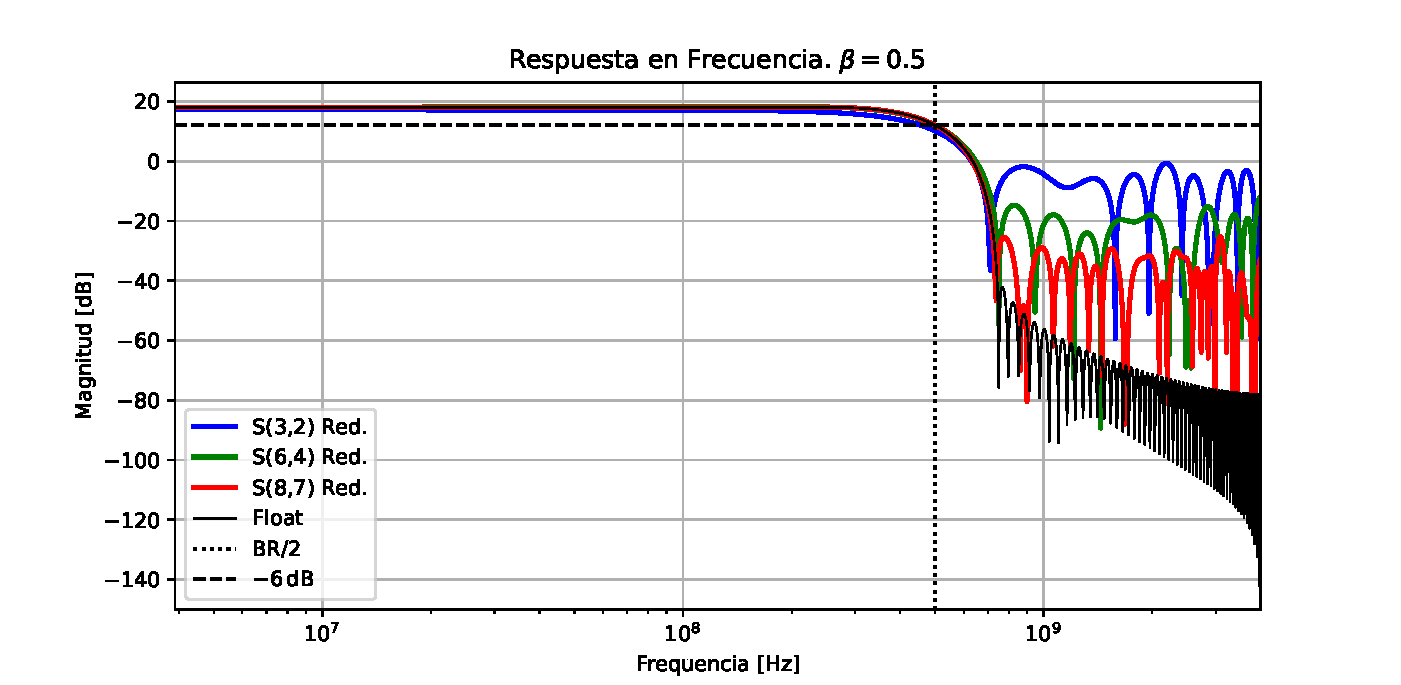
\includegraphics[width=\linewidth]{img/freq_fix_beta05_round.pdf}
    \caption{Respuesta en frecuencia del RC en punto fijo, con redondeo.}
    \label{fig:freq_fix_beta05_round}
\end{figure}

La convolución de estos filtros con los símbolos generan resultados como los de las figuras \ref{fig:conv_fix_s87}, \ref{fig:conv_fix_s64} y \ref{fig:conv_fix_s32}. 

En la figura \ref{fig:conv_fix_s87} se observa que el filtro de S(8,7) tiene relativamente una buena resolución, pudiendo adquirir un valor muy similar al del símbolo en el instante de muestreo; no es igual, ya que los coeficientes no llegan a 1 como se vio anteriormente.

En la figura \ref{fig:conv_fix_s64}, la degradación empieza a hacerse más notoria debido a la cuantización. En el caso de un filtro S(6,4) con redondeo, los valores son siempre iguales a los del símbolo debido al mayor rango de los coeficientes y su simetría.

\begin{figure}[H]
    \centering

    \begin{minipage}{0.48\linewidth}
        \centering
        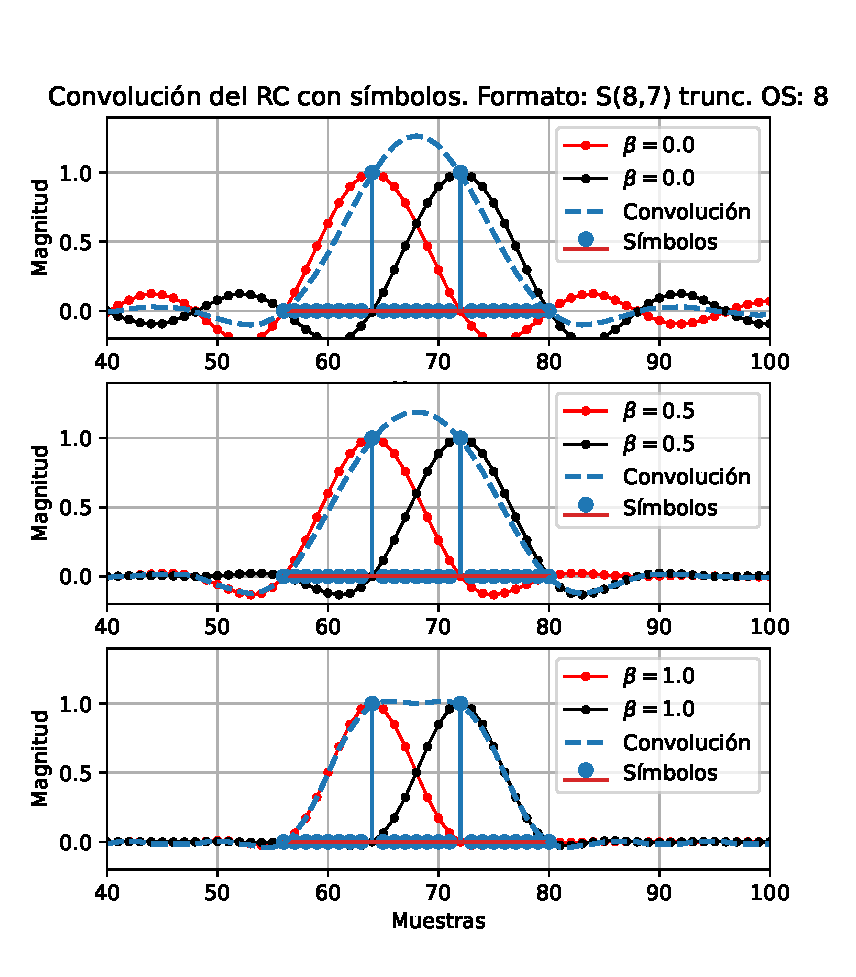
\includegraphics[width=1\linewidth]{img/conv_fix_s87_trunc.pdf}
    \end{minipage}
    \hfill
    \begin{minipage}{0.48\linewidth}
        \centering
        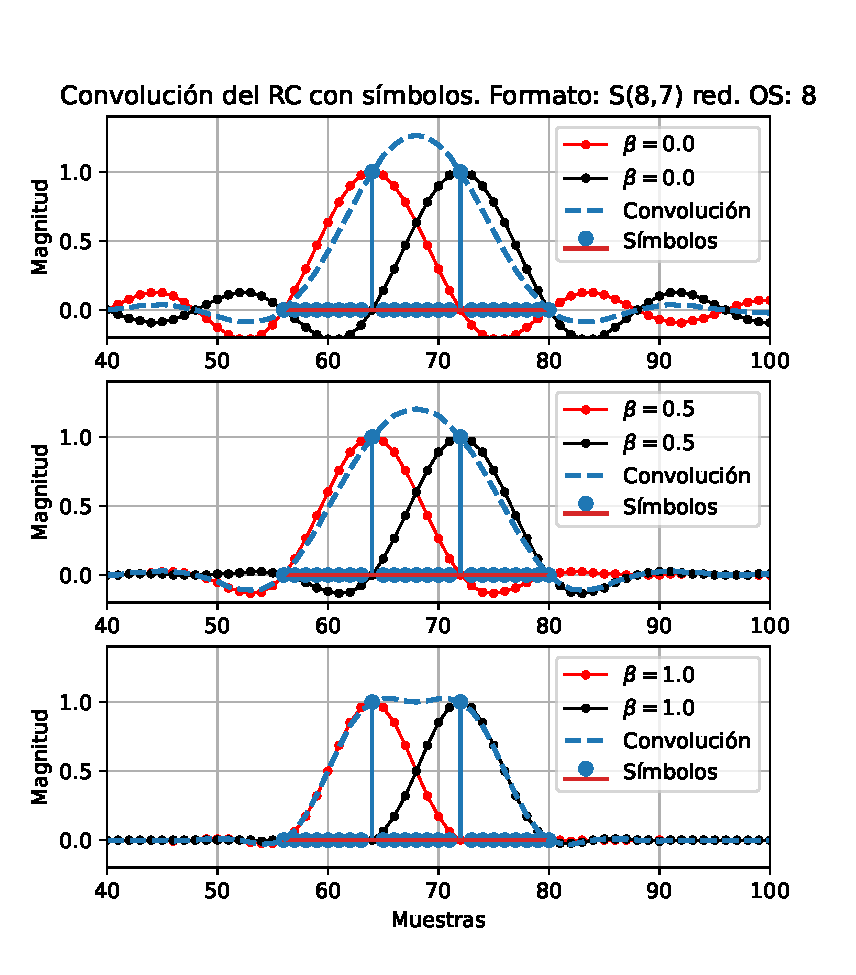
\includegraphics[width=1\linewidth]{img/conv_fix_s87_round.pdf}
    \end{minipage}

    \caption{Convolución del filtro en S(8,7) con dos símbolos.}
    \label{fig:conv_fix_s87}
\end{figure}

\begin{figure}[H]
    \centering

    \begin{minipage}{0.48\linewidth}
        \centering
        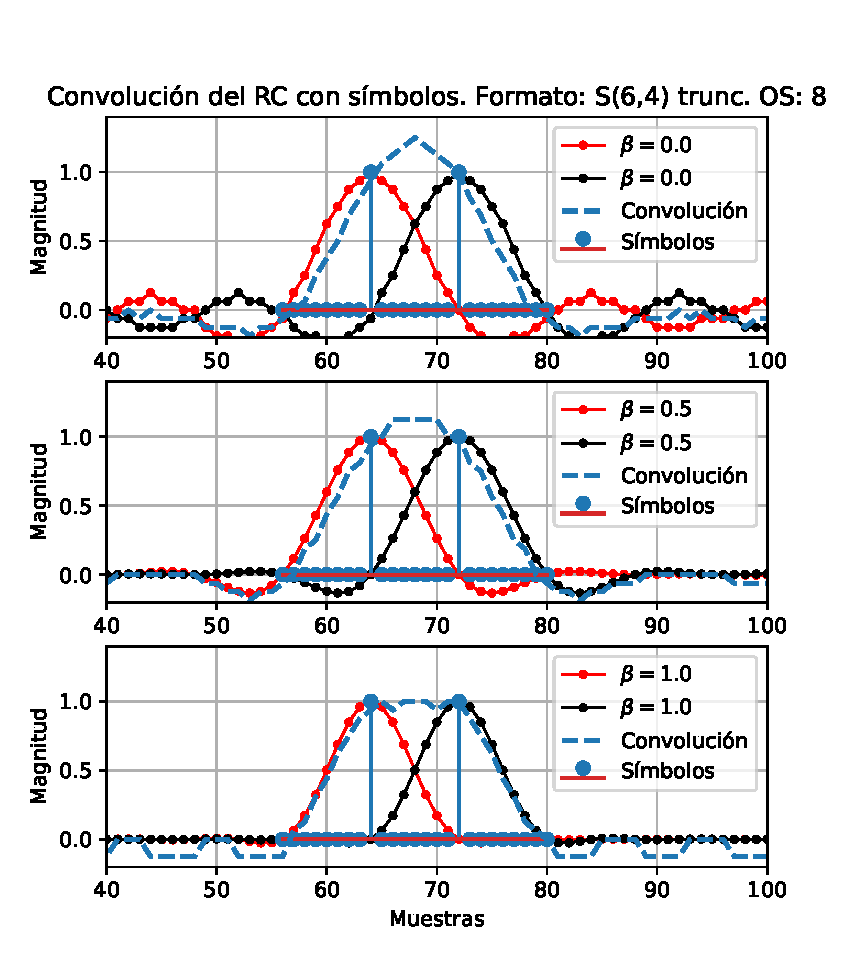
\includegraphics[width=1\linewidth]{img/conv_fix_s64_trunc.pdf}
    \end{minipage}
    \hfill
    \begin{minipage}{0.48\linewidth}
        \centering
        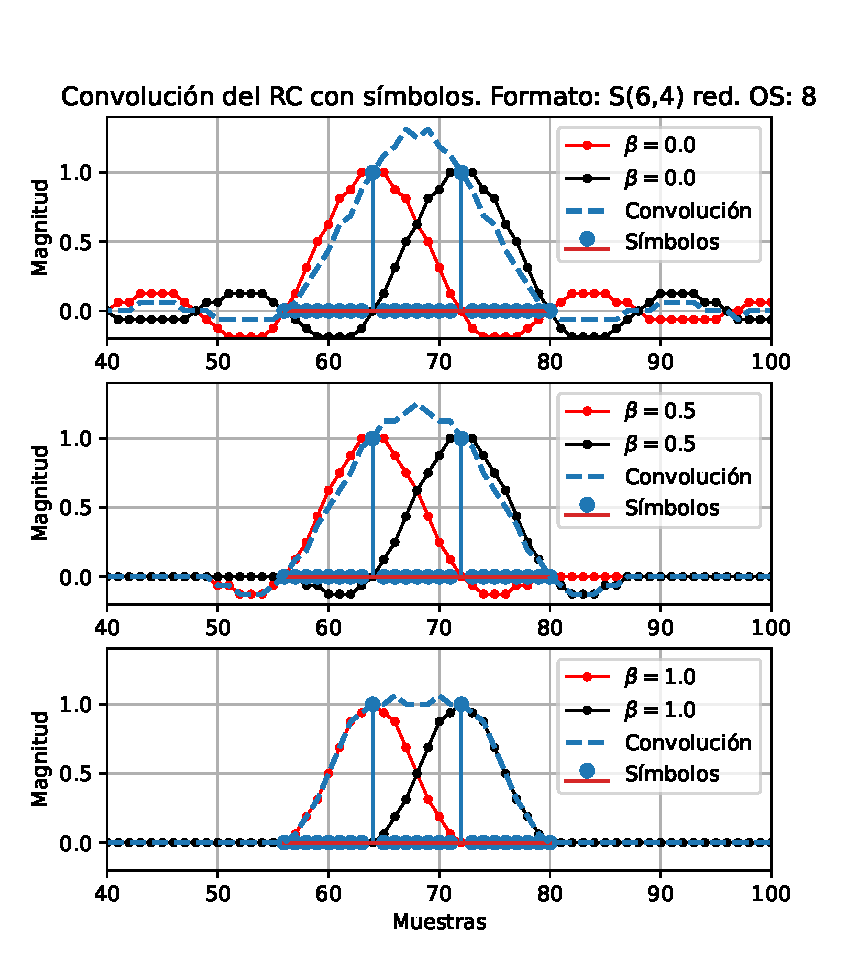
\includegraphics[width=1\linewidth]{img/conv_fix_s64_round.pdf}
    \end{minipage}

    \caption{Convolución del filtro en S(6,4) con dos símbolos.}
    \label{fig:conv_fix_s64}
\end{figure}

En el caso del filtro en S(3,2) de la figura \ref{fig:conv_fix_s32}, la degradación es muy alta y probablemente no se puedan detectar correctamente los símbolos a la hora del muestreo. 

En el script se generó una secuencia pseudoaleatoria de varios símbolos y se los convolucionó con todos los filtros cuantizados, luego se realizó el muestreo en la fase óptima y se graficó la constelación resultante. El resultado se muestra en las figuras \ref{fig:const_trunc} y \ref{fig:const_round}.

\begin{figure}[b!]
    \centering

    \begin{minipage}{0.48\linewidth}
        \centering
        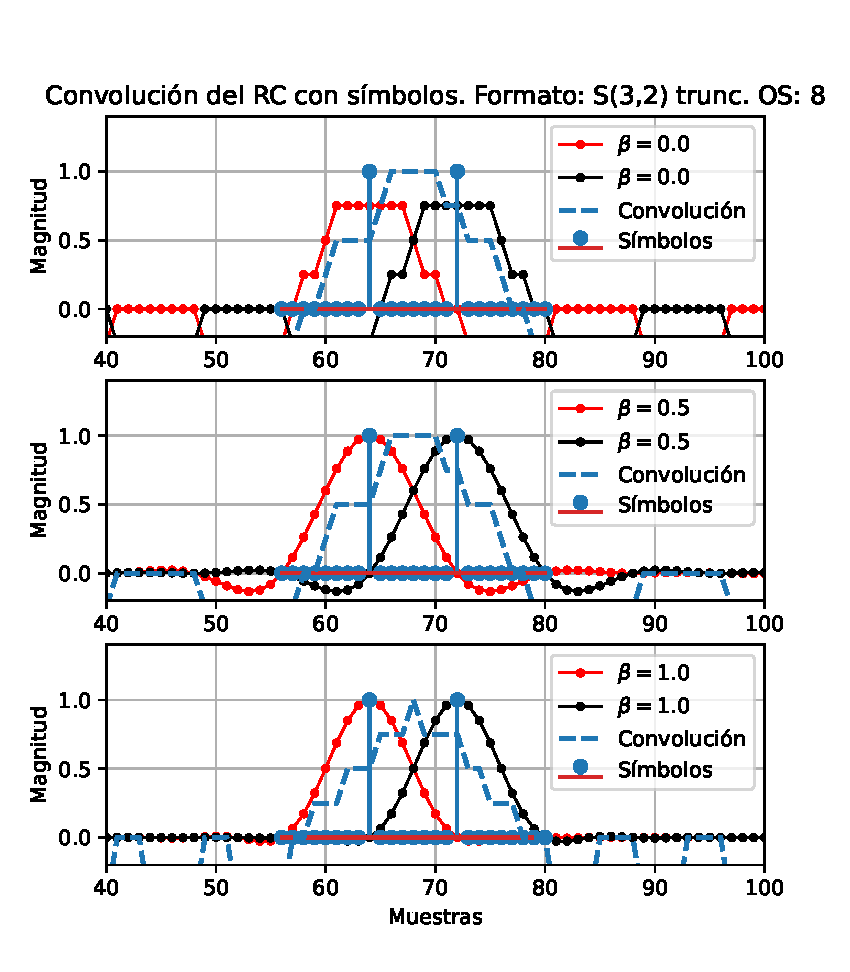
\includegraphics[width=1\linewidth]{img/conv_fix_s32_trunc.pdf}
    \end{minipage}
    \hfill
    \begin{minipage}{0.48\linewidth}
        \centering
        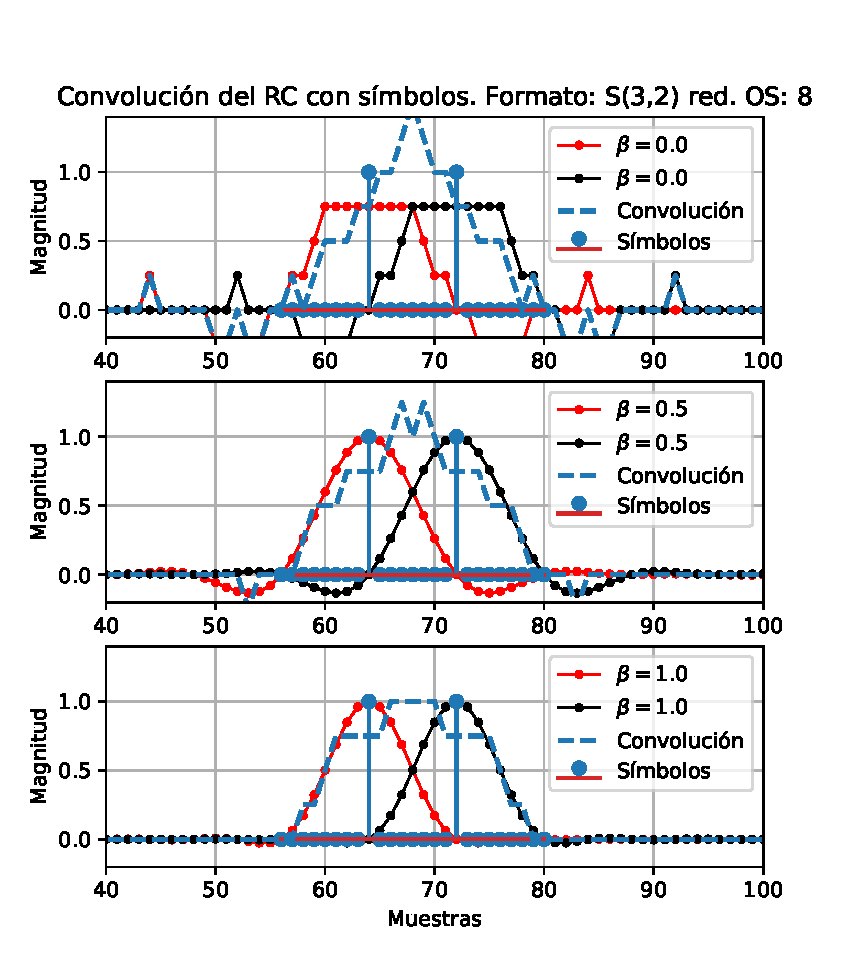
\includegraphics[width=1\linewidth]{img/conv_fix_s32_round.pdf}
    \end{minipage}

    \caption{Convolución del filtro en S(3,2) con dos símbolos.}
    \label{fig:conv_fix_s32}
\end{figure} 

Cuando el filtro se cuantiza con truncado, las muestras obtenidas son muy dispersas si la resolución es muy baja, resultando en un filtro con mal desempeño. En este caso el filtro en S(8,7) muestra un buen resultado para ser utilizado en un transmisor, mientras que con el filtro S(6,4), a pesar de que los símbolos caen dentro de la región de decisión correcta, el ruido aditivo de un canal real expande aún más esa ``nube'' de símbolos y genera errores en la decisión. Finalmente, el filtro en S(3,2) ya genera errores en la decisión, por lo que directamente no es útil.

Nótese, por otro lado, que el factor de rolloff no afecta la constelación, solo afecta el ancho de banda utilizado y la cantidad de coeficientes necesaria.

\begin{figure}[t!]
    \centering
    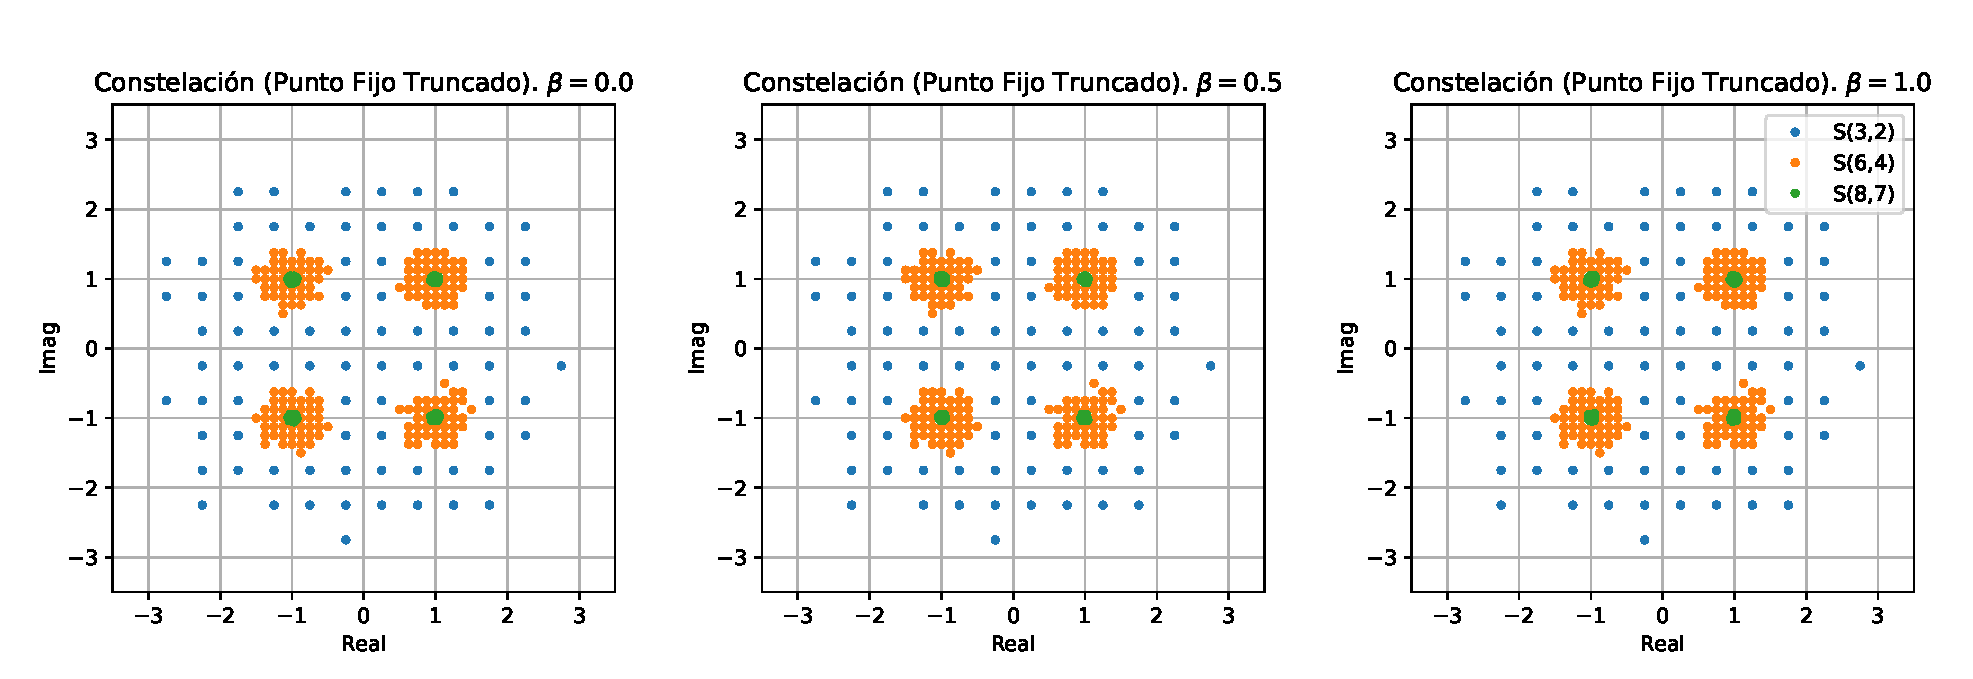
\includegraphics[width=\linewidth]{img/const_trunc.pdf}
    \caption{Diagrama de constelación para los filtros en punto fijo con truncado.}
    \label{fig:const_trunc}
\end{figure}

Si los filtros se cuantizan con redondeo, los símbolos que se muestrean caen mucho más cerca del valor correcto y sobre la región de decisión correcta. Sin embargo, en el caso del filtro en S(3,2) las muestras están más cerca del valor umbral de decisión, lo que genera una desventaja a la hora de transmitir en un canal con ruido aditivo.

\begin{figure}[t!]
    \centering
    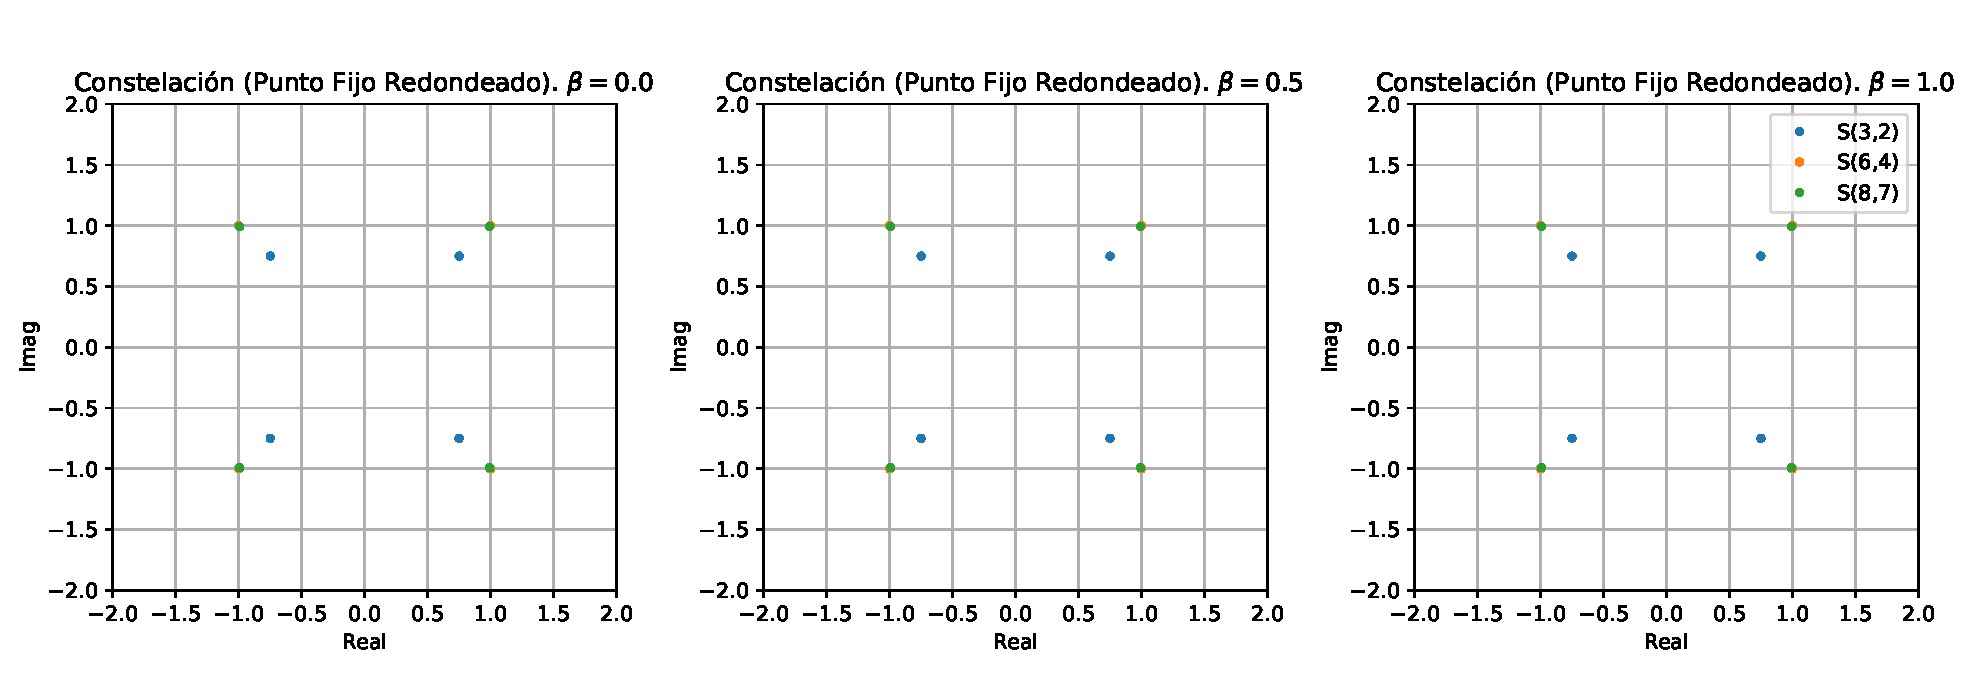
\includegraphics[width=\linewidth]{img/const_round.pdf}
    \caption{Diagrama de constelación para los filtros en punto fijo con redondeo.}
    \label{fig:const_round}
\end{figure}

\section{Conclusión}

Comparando los tres formatos de punto fijo propuestos, se concluye que S(8,7) es el formato que mejor sigue la respuesta ideal de un filtro RC, tanto en el dominio temporal como en el de frecuencia. Los coeficientes no llegan a 1 por la limitación de rango, pero la degradación es mínima. El formato S(6,4) es el de mayor rango, pero provoca muestras dispersas en la constelación si se utiliza el truncado; con redondeo, los valores muestreados coinciden con los del símbolo transmitido. Finalmente, el formato S(3,2) tiene una respuesta muy distinta a la ideal; con truncado, genera una gran dispersión en la constelación, y con redondeo, las muestras están más cerca del umbral de decisión, por lo que es inutilizable en la práctica.

Se observó, por otro lado, que el redondeo produce coeficientes simétricos, mejora la atenuación fuera de banda y mantiene una banda de paso más constante. El truncado, en cambio, rompe la simetría del filtro y degrada más la respuesta en frecuencia.

\appendix

\section{Scripts de Python} \label{appx:scripts}

Los scripts del trabajo se encuentran en el siguiente link: 

\noindent
\url{https://github.com/Ruben-Zuniga/Introduccion-al-Disenio-Digital/tree/main/TP3}

% \begin{equation}
%     \boxed{
%         1 = 2
%     }
% \end{equation}

% \begin{table}[H]
%     \centering

%     \begin{tabular}{lcc}
%         \textbf{A} & \textbf{B} & \textbf{C} \\
%         \hline\hline
%         A & B & C \\
%         A & B & C \\
%         \hline
%     \end{tabular}

%     \caption{cap.}
%     \label{tab:tab}
% \end{table}

% \begin{table}[H]
%     \centering
%     \begin{tblr}{
%         row{1} = {Titulo},
%         column{1} = {Titulo},
%         colspec = {Q[l] Q[c] Q[c]},
%         vlines,
%         hlines,
%         width=\linewidth
%     }
%         A & B & C \\
%         A & B & C \\
%         A & B & C \\

%     \end{tblr}
%     \caption{cap.}
%     \label{tab:tab}
% \end{table}

% \begin{figure}[H]
%     \centering
%     \includegraphics[width=0.85\linewidth]{img/sim.png}
%     \caption{cap.}
%     \label{fig:fig}
% \end{figure}

% \begin{figure}[H]
%     \centering

%     \begin{minipage}{0.48\linewidth}
%         \centering
%         \includegraphics[width=1\linewidth]{img/ondas_completo1.png}
%     \end{minipage}
%     \hfill
%     \begin{minipage}{0.48\linewidth}
%         \centering
%         \includegraphics[width=1\linewidth]{img/ondas_completo2.png}
%     \end{minipage}

%     \caption{cap.}
%     \label{fig:fig}
% \end{figure}

% \begin{figure}[H]
%     \centering

%     \begin{minipage}{\linewidth}
%         \centering
%         
\includegraphics[width=1\linewidth]{img/fulgor_logo.jpg}
%         \subcaption{cap.}
%         \label{fig:fig}
%     \end{minipage}
    
%     \begin{minipage}{\linewidth}
%         \centering
%         
\includegraphics[width=1\linewidth]{img/fulgor_logo.jpg}
%         \subcaption{cap.}
%         \label{fig:fig}
%     \end{minipage}
    
%     \begin{minipage}{\linewidth}
%         \centering
%         
\includegraphics[width=1\linewidth]{img/fulgor_logo.jpg}
%         \subcaption{cap.}
%         \label{fig:fig}
%     \end{minipage}

%     \caption{cap.}
%     \label{fig:fig}
% \end{figure}